\chapter{Estimación de Costos y Presupuesto}

\section{Resumen Financiero del Proyecto}
El desarrollo de esta investigación implica la implementación de una arquitectura híbrida de hardware y software para la validación de métricas ambientales. La estructura de costos se ha diseñado bajo el principio de eficiencia, priorizando el desarrollo de capital intelectual y la validación experimental sobre la adquisición de activos fijos costosos.

El presupuesto global estimado asciende a $267$ millones de pesos colombianos (COP), ejecutados a lo largo de 4 años. Este monto cubre desde la fase de diseño conceptual hasta la validación en campo y la divulgación científica.
\section{Desglose de Costos de Desarrollo Tecnológico}

A continuación se detalla la inversión específica requerida para la construcción del prototipo funcional (TRL 5-6), diferenciando componentes físicos y servicios digitales.

\begin{table}[H]
    \centering
    \begin{tabular}{|p{7cm}|c|c|}
        \hline
        \textbf{Componente Tecnológico} & \textbf{Unidades} & \textbf{Costo (MM COP)} \\ \hline
        \multicolumn{3}{|l|}{\textit{\textbf{1. Hardware y Sensórica (Nodo IoT)}}} \\ \hline
        Sensores de \ce{CO2} (NDIR Grado Industrial) & 3 & 0.6 \\ \hline
        Sensores de Gases Traza (\ce{CH4}, VOCs) & 3 & 0.72 \\ \hline
        Sensores Ambientales (Temp/Humedad de alta precisión) & 3 & 1.2 \\ \hline
        Sensores Auxiliares (Luz, pH, NPK) & 3 & 0.6 \\ \hline
        Unidades de Procesamiento (ESP32 + LoRa) & 5 & 4.0 \\ \hline
        Manufactura de PCB y Carcasas IP65 & 3 & 0.8 \\ \hline
        \multicolumn{3}{|l|}{\textit{\textbf{2. Software e Infraestructura de Datos}}} \\ \hline
        Desarrollo de Algoritmos Híbridos (Licenciamiento) & Global & 4.0 \\ \hline
        Interfaz de Visualización (Dashboard Web) & Global & 2.0 \\ \hline
        Infraestructura Cloud (Hosting + DB - 12 meses) & Global & 2.4 \\ \hline
        \multicolumn{3}{|l|}{\textit{\textbf{3. Validación y Transferencia}}} \\ \hline
        Equipos Patrón de Referencia (Alquiler/Uso) & Global & 2.0 \\ \hline
        Insumos para Ensayos Experimentales & Global & 2.8 \\ \hline
        Kit de Comunicaciones (Gateway LoRaWAN + Antenas) & 1 & 1.8 \\ \hline
        \multicolumn{3}{|l|}{\textit{\textbf{4. Servicios Especializados}}} \\ \hline
        Consultoría Técnica Externa & Global & 6.0 \\ \hline
        Capacitación y Formación Especializada & Global & 3.2 \\ \hline
        \textbf{SUBTOTAL DESARROLLO TECNOLÓGICO} & & \textbf{\$ 32.12} \\ \hline
    \end{tabular}
    \caption{Estimación de costos directos de desarrollo e implementación.}
    \label{tab:costos_desarrollo}
\end{table}

\section{Cronograma de Ejecución Financiera}

La siguiente tabla detalla la distribución de recursos por actividad estratégica, indicando el estado actual de avance y la valoración económica de los entregables (recursos humanos, técnicos y operativos).

\begin{longtable}{|p{5cm}|p{6cm}|c|c|}
    \hline
    \textbf{Actividad} & \textbf{Descripción del Rubro} & \textbf{\% Avance} & \textbf{Costo (MM COP)*} \\
    \hline
    \endfirsthead
    \multicolumn{4}{c}{\textit{Continúa de la página anterior}} \\
    \hline
    \textbf{Actividad} & \textbf{Descripción} & \textbf{\% Avance} & \textbf{Costo (MM COP)} \\
    \hline
    \endhead
    \hline
    \multicolumn{4}{r}{\textit{*MM COP: Millones de Pesos Colombianos}} \\
    \endfoot
    \hline
    \endlastfoot
    
    Revisión bibliográfica & Acceso a bases de datos y análisis del estado del arte. & 50\% & 6.0 \\
    \hline
    Infraestructura Computacional & Uso de equipos de cómputo, licencias de software y simulación. & 70\% & 8.0 \\
    \hline
    Ingeniería de Software & Desarrollo de algoritmos de backend y procesamiento (4 años). & 45\% & 20.0 \\
    \hline
    Ingeniería de Hardware & Diseño PCB, integración de sensores y manufactura de nodos. & 100\% & 20.0 \\
    \hline
    \textbf{Estudio Doctoral} & \textbf{Dedicación del investigador (Matrícula + Manutención 4 años).} & 45\% & 80.0 \\
    \hline
    Validación Experimental & Logística de campo, insumos biológicos (larvas) y sustratos. & 0\% & 16.0 \\
    \hline
    Desarrollo de IA & Entrenamiento de modelos y horas de procesamiento en GPU. & 10\% & 24.0 \\
    \hline
    Sistema MRV & Diseño de la plataforma de reporte y validación ambiental. & 60\% & 12.0 \\
    \hline
    Servicios en la Nube & Costos operativos de almacenamiento y despliegue (AWS/Azure). & 50\% & 10.0 \\
    \hline
    Divulgación Científica & Publicación en revistas y asistencia a congresos. & 25\% & 8.0 \\
    \hline
    Gestión del Proyecto & Administración, papelería y costos indirectos. & 60\% & 8.0 \\
    \hline
    Metrología y Calibración & Servicios de laboratorio certificado para validación de sensores. & 40\% & 12.0 \\
    \hline
    Escritura y Edición & Elaboración de documentos, traducción y corrección de estilo. & 20\% & 8.0 \\
    \hline 
    \textbf{TOTAL ESTIMADO} &  & \textbf{-} & \textbf{\$ 232.0} \\
    \hline
\end{longtable}

\section{Estrategia de Financiamiento}

La viabilidad financiera del proyecto se sustenta en un modelo mixto de financiación:

\begin{itemize}
    \item \textbf{Aporte Institucional (UNAL):} Cubre principalmente los costos de capital humano (dirección de tesis), acceso a laboratorios, infraestructura física y recursos bibliográficos, valorados como contrapartida en especie.
    \item \textbf{Recursos Propios:} El investigador asume los costos directos de adquisición de componentes electrónicos importados, insumos de experimentación y gastos operativos de campo no cubiertos por convocatorias institucionales.
\end{itemize}
\section{Cronograma de Actividades}

El plan de trabajo se estructura en un horizonte temporal de cuatro años (48 meses), organizado en cuatro fases secuenciales e interdependientes que garantizan el cumplimiento de los objetivos específicos. La distribución temporal de las actividades, detallada en la Figura \ref{fig:cronograma}, sigue una lógica incremental de desarrollo tecnológico y validación científica:

\begin{description}
    \item[Fase 1: Fundamentación y Diseño (Meses 1-12):] 
    Se centra en la revisión sistemática del estado del arte y la definición de la arquitectura del sistema. Incluye el diseño conceptual de los nodos IoT y el despliegue inicial de la infraestructura en la nube para asegurar la capacidad de almacenamiento de datos.
    
    \item[Fase 2: Desarrollo Tecnológico e Instrumentación (Meses 12-24):] 
    Etapa de ingeniería intensiva. Comprende la manufactura de los nodos sensores, la programación del firmware (Edge) y el desarrollo de la plataforma de software (Backend/Frontend). Finaliza con la puesta a punto de los protocolos de calibración de sensores.
    
    \item[Fase 3: Modelado e Inteligencia Híbrida (Meses 24-36):] 
    Núcleo científico de la tesis. Con los datos recolectados por los prototipos, se parametrizan los modelos mecanísticos (EDO) y se entrenan los algoritmos de aprendizaje automático para la corrección de errores y detección de anomalías.
    
    \item[Fase 4: Validación, MRV y Cierre (Meses 36-48):] 
    Ejecución de los ensayos experimentales finales para validar la precisión del sistema híbrido. Se consolida el módulo de reporte ambiental (MRV), se redactan los artículos científicos de alto impacto y se finaliza el documento de tesis doctoral.
\end{description}

De manera transversal, se contemplan actividades permanentes de gestión del proyecto y costos asociados a mediciones, asegurando la viabilidad operativa durante todo el ciclo de investigación.

\begin{sidewaysfigure}
    \centering
    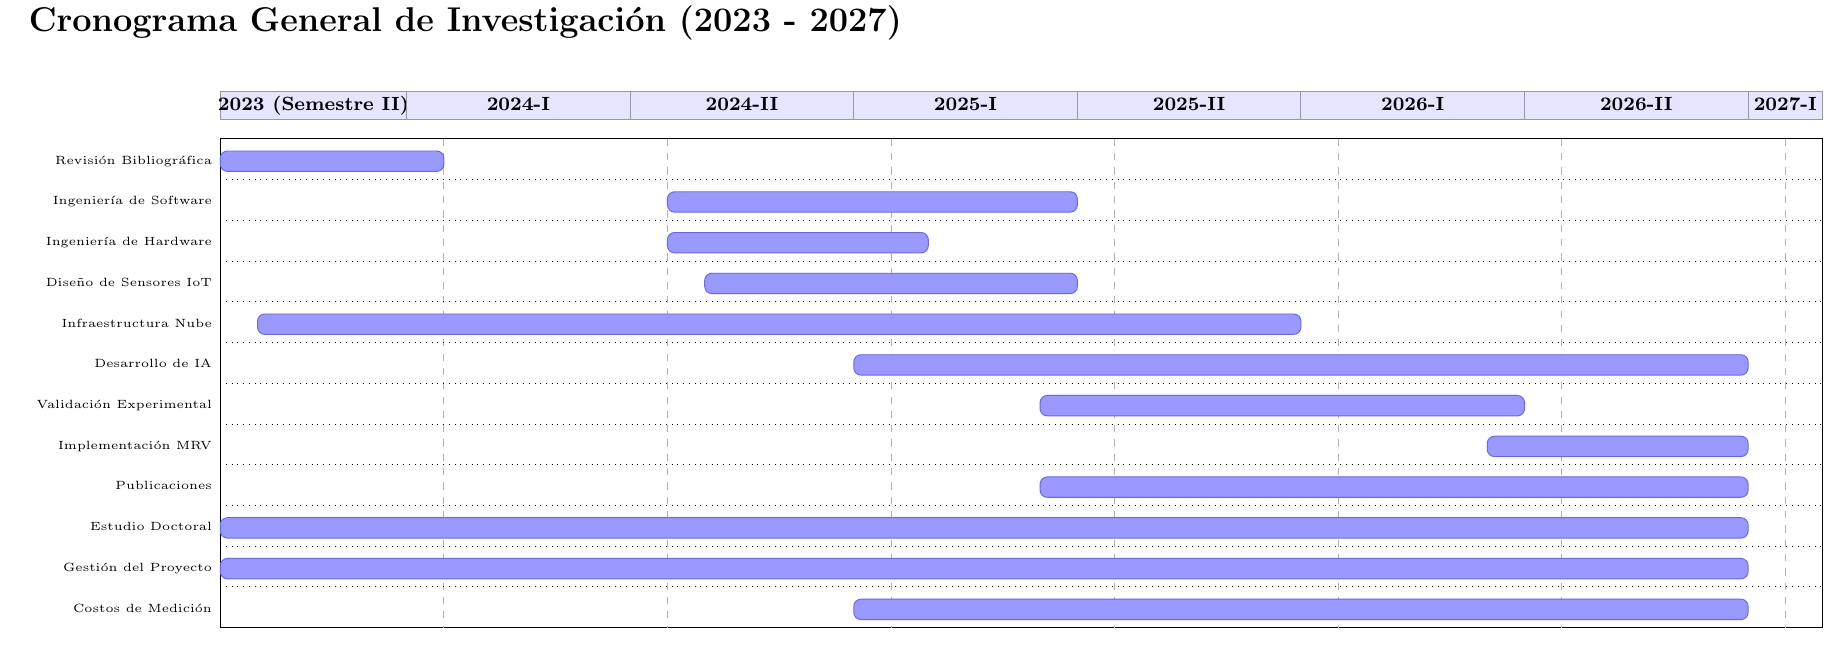
\includegraphics[width=1.0\textwidth]{00Figuras/gant.png}
    \caption{Cronograma detallado de actividades de investigación (2023-2027).}
    \label{fig:cronograma}
\end{sidewaysfigure}

\section{Retorno de la Inversión (Justificación)}
Más allá del aporte académico, la inversión en este sistema genera valor tangible al reducir la incertidumbre en la medición de emisiones. Un sistema MRV validado habilita el acceso a mercados de carbono, cuyo potencial económico para una planta de bioconversión de 10 toneladas/día podría superar los costos de implementación tecnológica en menos de 2 años de operación, demostrando la sostenibilidad financiera de la propuesta a escala industrial.

